%%%%%%%%%%%%%%%%%%%%%%%%%%%%%%%%%%%%%%%%%%%%%%%%%%%%%%%%%%%%%%%%%%%%%%%%%%%%%%%%
%%%%%%%%%%%%%%%%%%%%%%%%%%%%%%%%%%%%%%%%%%%%%%%%%%%%%%%%%%%%%%%%%%%%%%%%%%%%%%%%
%%                                                                            %%
%% thesistemplate.tex version 4.00 (2023/02/09)                               %%
%% The LaTeX template file to be used with the aaltothesis.sty (version 4.00) %%
%% style file.                                                                %%
%% This package requires pdfx.sty v. 1.5.84 (2017/05/18) or newer.            %%
%%                                                                            %%
%% This is licensed under the terms of the MIT license below.                 %%
%%                                                                            %%
%% Written by Luis R.J. Costa.                                                %%
%% Currently developed at Teacher services, Learning Services of Aalto        %%
%% University by Luis R.J. Costa since May 2019.                              %%
%%                                                                            %%
%% Copyright 2017-2021 aaltothesis.cls by Luis R.J. Costa,                    %%
%% luis.costa@aalto.fi.                                                       %%
%% Copyright 2017-2018 Swedish translations in aaltothesis.cls by Elisabeth   %%
%% Nyberg and Henrik Wallén henrik.wallen@aalto.fi.                           %%
%% Finnish documentation in the template opinnatepohja.tex translated from    %%
%% the English template documentation.                                        %%
%% Copyright 2021 English template thesistemplate.tex by Luis R.J. Costa,     %%
%% Maurice Forget, Henrik Wallén.                                             %%
%% Copyright 2018-2022 Swedish template kandidatarbetsbotten.tex by Henrik    %%
%% Wallen.                                                                    %%
%%                                                                            %%
%% Permission is hereby granted, free of charge, to any person obtaining a    %%
%% copy of this software and associated documentation files (the "Software"), %%
%% to deal in the Software without restriction, including without limitation  %%
%% the rights to use, copy, modify, merge, publish, distribute, sublicense,   %%
%% and/or sell copies of the Software, and to permit persons to whom the      %%
%% Software is furnished to do so, subject to the following conditions:       %%
%% The above copyright notice and this permission notice shall be included in %%
%% all copies or substantial portions of the Software.                        %%
%% THE SOFTWARE IS PROVIDED "AS IS", WITHOUT WARRANTY OF ANY KIND, EXPRESS OR %%
%% IMPLIED, INCLUDING BUT NOT LIMITED TO THE WARRANTIES OF MERCHANTABILITY,   %%
%% FITNESS FOR A PARTICULAR PURPOSE AND NONINFRINGEMENT. IN NO EVENT SHALL    %%
%% THE AUTHORS OR COPYRIGHT HOLDERS BE LIABLE FOR ANY CLAIM, DAMAGES OR OTHER %%
%% LIABILITY, WHETHER IN AN ACTION OF CONTRACT, TORT OR OTHERWISE, ARISING    %%
%% FROM, OUT OF OR IN CONNECTION WITH THE SOFTWARE OR THE USE OR OTHER        %%
%% DEALINGS IN THE SOFTWARE.                                                  %%
%%                                                                            %%
%%                                                                            %%
%%%%%%%%%%%%%%%%%%%%%%%%%%%%%%%%%%%%%%%%%%%%%%%%%%%%%%%%%%%%%%%%%%%%%%%%%%%%%%%%
%%                                                                            %%
%%                                                                            %%
%% An example for writting your thesis using LaTeX                            %%
%% Original version and development work by Luis Costa, changes to the text   %%
%% in the Finnish template by Perttu Puska.                                   %%
%% Support for Swedish added 15092014                                         %%
%% PDF/A-b support added on 15092017                                          %%
%% PDF/A-2 support added on 24042018                                          %%
%% Layout design and typesettin changed 15072021                              %%
%%                                                                            %%
%% This example consists of the files                                         %%
%%       thesistemplate.tex (version 4.00) (for text in English)              %%
%%       opinnaytepohja.tex (version 4.00) (for text in Finnish)              %%
%%       kandidatarbetsbotten.tex (version 1.10) (for text in Swedish)        %%
%%       aaltothesis.cls                                                      %%
%%       linediagram.pdf (graphics file)                                      %%
%%       curves.pdf      (graphics file)                                      %%
%%       ledspole.jpg    (graphics file)                                      %%
%%                                                                            %%
%%                                                                            %%
%% Typeset in Linux with                                                      %%
%% pdflatex: (recommended method)                                             %%
%%             $ pdflatex thesistemplate                                      %%
%%             $ pdflatex thesistemplate                                      %%
%%                                                                            %%
%%   The result is the file thesistemplate.pdf that is PDF/A compliant, if    %%
%%   you have chosen the proper \documenclass options (see comments below)    %%
%%   and your included graphics files have no problems.                       %%
%%                                                                            %%
%%                                                                            %%
%% Explanatory comments in this example begin with the characters %%, and     %%
%% changes that the user can make with the character %                        %%
%%                                                                            %%
%%%%%%%%%%%%%%%%%%%%%%%%%%%%%%%%%%%%%%%%%%%%%%%%%%%%%%%%%%%%%%%%%%%%%%%%%%%%%%%%
%%%%%%%%%%%%%%%%%%%%%%%%%%%%%%%%%%%%%%%%%%%%%%%%%%%%%%%%%%%%%%%%%%%%%%%%%%%%%%%%
%%
%% WHAT is PDF/A
%%
%% PDF/A is the ISO-standardized version of the pdf. The standard's goal is to
%% ensure that he file is reproducable even after a long time. PDF/A differs
%% from pdf in that it allows only those pdf features that support long-term
%% archiving of a file. For example, PDF/A requires that all used fonts are
%% embedded in the file, whereas a normal pdf can contain only a link to the
%% fonts in the system of the reader of the file. PDF/A also requires, among
%% other things, data on colour definition and the encryption used.
%% Currently three PDF/A standards exist:
%% PDF/A-1: based on PDF 1.4, standard ISO19005-1, published in 2005.
%%          Includes all the requirements essential for long-term archiving.
%% PDF/A-2: based on PDF 1.7, standard ISO19005-2, published in 2011.
%%          In addition to the above, it supports embedding of OpenType fonts,
%%          transparency in the colour definition and digital signatures.
%% PDF/A-3: based on PDF 1.7, standard ISO19005-3, published in 2012.
%%          Differs from the above only in that it allows embedding of files in
%%          any format (e.g., xml, csv, cad, spreadsheet or wordprocessing
%%          formats) into the pdf file.
%% PDF/A-4: based on PDF 2.0, standard ISO19005-4, published in November 2020.
%%
%% PDF/A-1 files are not necessarily PDF/A-2 -compatible and PDF/A-2 are not
%% necessarily PDF/A-1 -compatible.
%% Standards PDF/A-1, PDF/A-2 and PDF/A-3 have two levels:
%% b: (basic) requires that the visual appearance of the document is reliably
%%    reproduceable.
%% a (accessible) in addition to the b-level requirements, specifies how
%%   accessible the pdf file is to assistive software, say, for the physically
%%   impaired.
%% The PDF/A-4 standard does not have additional levels like in the earlier
%% standards.
%% For more details on PDF/A, see, e.g.,
%% https://www.loc.gov/preservation/digital/formats/fdd/fdd000318.shtml or
%% https://www.pdfa.org/resource/iso-19005-pdfa/
%%
%%
%% WHICH PDF/A standard should my thesis conform to?
%%
%% Either to the PDF/A-1b or the PDF/A-2b standard. If all the figures and
%% graphs used in thesis work do not require transparency features, use either
%% PDF/A-1b or PFDF/A-2b. If you have figures with transparency
%% characteristics, use the PDF/A-2b standard. However, drawing applications
%% often use the transparency parameter, setting it to zero, to specify opacity
%% and get the basic 2-D visualisation. As a result, validation of PDF/A-1b
%% will fail. Use PDF/A-2b if PDF/A-1b validation fails.
%% Do not use the PDF/A-3b standard for your thesis.
%% The font to be used are specified in this templatenand they should not be
%% changed. In addition to not adhering to Aalto's visual guidelines, you may
%% have difficulties in producing a PDF/A-compliant PDF.
%%
%%
%% Validate your PDF/A file at https://www.pdf-online.com/osa/validate.aspx
%%
%%
%% WHAT graphics format can I use to produce my PDF/A compliant file?
%%
%% When using pdflatex to compile your work, favour the use of pdf, but you can
%% use the jpg or png format especially for photographs. You will have PDF/A
%% compliance problems with figures in pdf if the fonts are not embedded in the
%% pdf file.
%% If you choose to use latex to compile your work, the only acceptable file
%% format for your figure is eps. DO NOT use the ps format for your figures.

%% USE one of the following three \documentclass set-ups:
%% * the first when using pdflatex to directly typeset your document in the
%%   chosen pdf/a format for online publishing (centred page layout),
%% * the second for one-sided printing your thesis with the layout (wide left
%%   margin), or
%% * the third for two-sided printing.
%%
\documentclass[english, 12pt, a4paper, sci, utf8, a-2b, online]{aaltothesis}
%\documentclass[english, 12pt, a4paper, sci, utf8, a-2b, print]{aaltothesis}
%\documentclass[english, 12pt, a4paper, sci, utf8, a-2b, print, twoside]{aaltothesis}

%% Use the following options in the \documentclass macro above:
%% your school: arts, biz, chem, elec, eng, sci
%% the character encoding scheme used by your editor: utf8, latin1
%% thesis language: english, finnish, swedish
%% make an archiveable PDF/A-1b or PDF/A-2b compliant file: a-1b, a-2b
%%                    (with pdflatex, a normal pdf containing metadata is
%%                     produced without the a-*b option)
%% typset for online document or print on paper: online, print
%%        online: typeset in symmetric layout and blue hypertext for online
%%                publishing
%%        print: typeset in a symmetric layout and black hypertext for printing
%%               on paper
%%          two-side printing: twoside (default is one-sided printing)
%%               typeset in a wide margin on the binding side of the page and
%%               black hypertext. Use with print only.
%%

%% Use one of these if you write in Finnish (or use the Finnish template
%% opinnaytepohja.tex)
%\documentclass[finnish, 12pt, a4paper, elec, utf8, a-1b, online]{aaltothesis}
%\documentclass[finnish, 12pt, a4paper, elec, utf8, a-1b, print]{aaltothesis}
%\documentclass[finnish, 12pt, a4paper, elec, utf8, a-1b, print, twoside]{aaltothesis}

%% Use one of these if you write in Swedish (or use the Swedish template
%% kandidatarbetsbotten.tex)
%\documentclass[swedish, 12pt, a4paper, elec, utf8, a-2b, online]{aaltothesis}
%\documentclass[swedish, 12pt, a4paper, elec, utf8, a-2b]{aaltothesis}
%\documentclass[swedish, 12pt, a4paper, elec, dvips, online]{aaltothesis}

%% FOR USERS OF AMS PACKAGES:
%% * newtxmath used in this template loads amsmath, so
%%   you needn't load it. If you want to use options in amsmath, load it here,
%%   before \setupthesisfonts below to pass the options to amsmath.
%% * If you want to use amsthm, load it here before \setupthesisfonts to avoid
%%   a clash with newtxmath.
%% * If using amsmath with options and you want to use amsthm, load amsthms
%%   after amsmath, as described in the amsthm documentation.
%% * Don't use amsbsym or amsfonts. The symbols [and macros] there are defined in
%%   newtxmath and so clash if used.
%\usepackage[options]{amsmath}
%\usepackage{amsthm}

%% DO NOT MOVE OR REMOVE \setupthesisfonts
\setupthesisfonts

%% Add here the packges you need
\usepackage{graphicx}
\usepackage{tabularx,ragged2e}
\newcolumntype{C}{>{\Centering\arraybackslash}X} % centered "X" column
\usepackage{enumitem}
\usepackage{float}

% \usepackage{amsfonts,amssymb,amsbsy,csquotes}
\usepackage{csquotes}
\usepackage{biblatex}
\addbibresource{./refs.bib}

% \usepackage{hyperref}
% \hypersetup{pdfpagemode=UseNone, pdfstartview=FitH,
%   colorlinks=true,urlcolor=red,linkcolor=blue,citecolor=black,
%   pdftitle={Default Title, Modify},pdfauthor={Your Name},
%   pdfkeywords={Modify keywords}}

%% For tables that span multiple pages; used to split a paraphrasing example in the appendix. If you don't need it, remove it.
\usepackage{longtable}

%% A package for generating Creative Commons copyright terms. If you don't use the CC copyright terms, remove it, since otherwise undesired information may be added to this document's metadata.
\usepackage[type={CC}, modifier={by-nc-sa}, version={4.0}]{doclicense}
%% Find below three examples for typesetting the CC license notice.

%% Edit to conform to your degree programme
%% Capitalise the words in the name of the degree programme: it's a name
\degreeprogram{Computer, Communication and Information Sciences}

%% Your major
\major{Computer Science}

%% Choose one of the three below
%\univdegree{BSc}
\univdegree{MSc}
%\univdegree{Lic}

\thesisauthor{Aarni Halinen}

%% Your thesis title and possible subtitle comes here and possibly, again, together with the Finnish or Swedish abstract. Do not hyphenate the title (and subtitle), and avoid writing too long a title. Should LaTeX typeset a long title (and/or subtitle) unsatisfactorily, you might have to force a linebreak using the \\ control characters. In this case...
%% * Remember, the title should not be hyphenated!
%% * A possible 'and' in the title should not be the last word in the line; it begins the next line.
%% * Specify the title (and/or subtitle) again without the linebreak characters in the optional argument in box brackets. This is done because the title is part of the metadata in the pdf/a file, and the metadata cannot contain linebreaks.
\thesistitle{Kubernetes inter-pod container isolation}
% \thesistitle[Title of the thesis]{Title of\\ the thesis}
%% Either remove or leave \thesissubtitle{} empty if you don't use it \thesissubtitle{A possible subtitle}
% \thesissubtitle{}

\place{Espoo}

%% The date for the bachelor's thesis is the day it is presented
\date{1 June 2023}

%% Thesis supervisor
%% Note the "\" character in the title after the period and before the space and the following character string. This is because the period is not the end of a sentence after which a slightly longer space follows, but what is desired is a regular interword space.
\supervisor{Prof.\ Mario Di Francesco}

%% Advisor(s)---two at the most---of the thesis. Check with your supervisor how many official advisors you can have.
\advisor{M.Sc.\ (Tech.)\ José\ Luis\ Martin\ Navarro}
\advisor{M.Sc.\ (Tech.)\ Jacopo\ Bufalino}

%% If you do your thesis work in a company of other institute, give the name of the company or instution here. Otherwise, leave the macro empty, comment it out, or remove it. This will remove this field from the abstract page.
% \collaborativepartner{Company or institute name}

%% Aaltologo: syntax:
%% \uselogo{?|!|''}
%% The logo language is set to be the same as the thesis language.
%\uselogo{?}
%\uselogo{!}
\uselogo{''}

%%%%%%%%%%%%%%%%%%               COPYRIGHT TEXT               %%%%%%%%%%%%%%%%%%
%%%%%%%%%%%%%%%%%%%%%%%%%%%%%%%%%%%%%%%%%%%%%%%%%%%%%%%%%%%%%%%%%%%%%%%%%%%%%%%%

%% Copyright of a work is with the creator/author of the work regardless of
%% whether the copyright mark is explicitly in the work or not. You may, if you
%% wish---we encourage you to do so---publish your work under a Creative
%% Commons license (see creativecommons.org), in which case the license text
%% must be visible in the work. Write here the copyright text you want using the
%% macro \copyrighttext, which writes the text into the metadata of the pdf file
%% as well.
%%
%% Syntax:
%% \copyrigthtext{metadata text}{text visible on the page}
%%
%% CHOOSE ONE OF THE COPYRIGHT NOTICE STYLES BELOW.
%% IF USING THE CC TERMS, CHOOSE THE LICENSE YOU WANT TO USE.
%% The different CC licenses are listed at
%% https://creativecommons.org/about/cclicenses/.
%% If you use the icons from the dolicense.sty package, add the package above
%% (\usepackage{dolicense}).
%% IMPORTANT NOTE!! Manually write the CC text in the \copyrighttext metadata
%% text field.
%%
%% NOTE: In the macros below, the text written in the metadata must have a
%% \noexpand macro before the \copyright special character. When not in pdf/a
%% mode (i.e. a-1b or a-2b are not specified in \documentclass), two \noexpands
%% are required in the metadata text to correctly render the copyright mark in
%% the pdf metadata. In pdf/a mode one \noexpand suffices.
%%
%% EXAMPLE OF PLAIN COPYRIGHT TEXT
%% The macros \copyright and \year below must be separated by the \ character
%% (space chacter) from the text that follows. The macros in the argument of the
%% \copyrighttext macro automatically insert the year and the author's name.
%% (Note! \ThesisAuthor is an internal macro of the aaltothesis.cls class file).
%%
%\copyrighttext{Copyright \noexpand\textcopyright\ \number\year\ \ThesisAuthor}
%{Copyright \textcopyright{} \number\year{} \ThesisAuthor}
%%
%% Of course, the same text could have simply been written as
%% \copyrighttext{Copyright \noexpand\copyright\ 2018 Eddie Engineer}
%% {Copyright \copyright{} 2022 Eddie Engineer}
%%
%% EXAMPLES OF CC LICENSE: different ways to display the same license
%% 1. A simple Creative Commons license text with a link to the copyright notice:
%\copyrighttext{\noexpand\textcopyright\ \number\year. This work is
%	licensed under a CC BY-NC-SA 4.0 license.}{\textcopyright{}
%	\number\year. This work is licensed under a
%	\href{https://creativecommons.org/licenses/by-nc-nd/4.0/}{CC BY-NC-SA 4.0}
%	license.}
%
%% To get the URL of the license of your choice, go to
%% https://creativecommons.org/about/cclicenses/, click on the chosen license
%% you want to use, and copy-and-paste the URL in the macro \href above.
%%
%% 2. A short Creative Commons license text containing the respective CC icons
%% (requires the package dolicense.sty to be added in the preamble as done
%% above) and a link to the corresponding Creative Commons license webpage (see
%% the dolicense package documentation for other license icons):
%\copyrighttext{\noexpand\textcopyright\ \number\year. This work is licensed
%	under a CC BY-NC-SA 4.0 license.}{
%	\parbox{95mm}{\noindent\textcopyright\ \number\year. \doclicenseText}
%	\hspace{1em}\parbox{35mm}{\doclicenseImage}
%}
%%
%% 3. An expanded Creative Commons license text containing the respective CC
%% icons text and as generated by the dolicense.sty package (the license is set
%% via package options in \usepackage[options]{dolicense} above; see the
%% dolicense package documentation for other license texts and icons):
\copyrighttext{\noexpand\textcopyright\ \number\year. This work is licensed under a Creative Commons "Attribution-NonCommercial-ShareAlike 4.0 International" (BY-NC-SA 4.0) license.}{\noindent\textcopyright\ \number \year \ \doclicenseThis}
%%%%%%%%%%%%%%%%%%%%%%%%%%%%%%%%%%%%%%%%%%%%%%%%%%%%%%%%%%%%%%%%%%%%%%%%%%%%%%%%


%% The English abstract:
%% All the details (name, title, etc.) on the abstract page appear as specified
%% above.
%% Thesis keywords:
%% Note! The keywords are separated using the \spc macro
\keywords{Kubernetes, Container, Docker, Security}

%% The abstract text. This text is included in the metadata of the pdf file as well as the abstract page.
\thesisabstract{
The abstract is a short description of the essential contents of the thesis:
what was studied and how and what were the main findings. For a Finnish thesis,
the abstract should be written in both Finnish and English; for a Swedish
thesis, in Swedish and English. The abstracts for English theses written by
Finnish or Swedish speakers should be written in English and either in Finnish
or in Swedish, depending on the student’s language of basic education. Students
educated in languages other than Finnish or Swedish write the abstract only in
English. Students may include a second or third abstract in their native
language, if they wish.
The abstract text of this thesis is written on the readable abstract page as
well as into the pdf file's metadata via the thesisabstract macro (see the
comment in the TeX file). Write here the text that goes into the metadata. The
metadata cannot contain special characters, linebreak or paragraph break
characters, so these must not be used here. If your abstract does not contain
special characters and it does not require paragraphs, you may take advantage of
the abstracttext macro (see the comment in the TeX file below). Otherwise, the
metadata abstract text must be identical to the text on the abstract page.
}

%% You can prevent LaTeX from writing into the xmpdata file (it contains all the metadata to be written into the pdf file) by setting the writexmpdata switch to 'false'. This allows you to write the metadata in the correct format directly into the file thesistemplate.xmpdata.
% \setboolean{writexmpdatafile}{false}

%% All that is printed on paper starts here
\begin{document}

%% Create the coverpage
\makecoverpage

%% Typeset the copyright text.
%% If you wish, you may leave out the copyright text from the human-readable page of the pdf file. This may seem like a attractive idea for the printed document especially if "Copyright (c) yyyy Eddie Engineer" is the only text on the page. However, the recommendation is to print this copyright text.
\makecopyrightpage

\clearpage
%% Note that when writing your thesis in English, place the English abstract first followed by the possible Finnish or Swedish abstract.

%% Abstract text
%% All the details (name, title, etc.) on the abstract page appear as specified above.

%% The text in the \thesisabstract macro is stored in the macro \abstractext, so you can use the text metadata abstract directly as follows:
\begin{abstractpage}[english]
  \abstracttext{}
\end{abstractpage}

%% Force a new page so that the possible Finnish or Swedish abstract does not begin on the same page
\newpage
%% Abstract in Finnish.  Delete if you don't need it.
%% Respecify those fields that differ from the earlier specification or simply respecify all fields.
\thesistitle{Opinnäyteen otsikko}
% \thesissubtitle{Opinnäytteen mahdollinen alaotsikko}
\supervisor{Prof.\ Mario Di Francesco}
\advisor{DI José\ Luis\ Martin\ Navarro}
\advisor{DI Jacopo\ Bufalino}
% \degreeprogram{Elektroniikka ja sähkötekniikka}
% \major{Sopiva pääaine}
% \collaborativepartner{Yhtiön tai laitoksen nimi}
\date{1.6.2023}
%% The keywords need not be separated by \spc now.
\keywords{Vastus, resistanssi, lämpötila}
%% Abstract text
\begin{abstractpage}[finnish]
Tiivistelmä on lyhyt kuvaus työn keskeisestä sisällöstä: mitä tutkittiin ja
miten sekä mitkä olivat tärkeimmät tulokset. Suomenkielisen opinnäytteen
tiivistelmä kirjoitetaan suomeksi ja englanniksi ja ruotsinkielisen vastaavasti
ruotsiksi ja englanniksi. Suomen- tai ruotsinkielisten opiskelijoiden, joiden
opinnäytteen kieli on englanti, tulee kirjoittaa tiivistelmänsä englanniksi ja
koulusivistyskielellään. Muiden kuin koulusivistyskieleltään suomen- tai
ruotsinkielisten tulee kirjoittaa tiivistelmänsä vain englanniksi. Opiskelija
voi halutessaan lisätä opinnäytteeseensä toisen tai kolmannen tiivistelmän
omalla äidinkielellään.
Tämän opinnäytteen tiivistelmäteksti kirjoitetaan opinnäytteen luettavan osan
lomakkeen lisäksi myös pdf-tiedoston metadataan. Kirjoita tähän metadataan
kirjoitettavaa teksti. Metadatatekstissa ei saa olla erikoismerkkejä,
rivinvaiho- tai kappaleenjakomerkkiä, joten näitä merkkeja ei saa käyttää tässä.
Jos tiivistelmäsi ei sisällä erikoimerkkejä eikä kaipaa kappaleenjakoa, voit
hyödynttää makroa abstracttext luodessasi lomakkeen tiivistelmää (katso
kommentti tässä TeX-tiedostossa alla). Metadatatiivistelmatekstin on muuten
oltava sama kuin lomakkeessa oleva teksti.

\end{abstractpage}

%% Force new page so that the Swedish abstract starts from a new page
\newpage

\dothesispagenumbering{}

%% Preface
%% This section is optional. Remove it if you do not want a preface.
\mysection{Preface}
% \mysection{Esipuhe}
I want to thank Professor Pirjo Professor and my instructors Dr Alan Advisor and
Ms Elsa Expert for their guidance.

I also want to thank my partner for keeping me sane and alive.

\vspace{5cm}
Otaniemi, 9 February 2023\\

\vspace{5mm}
{\hfill Aarni O.\ Halinen \hspace{1cm}}

%% Force a new page after the preface
\newpage

%% Table of contents.
\thesistableofcontents

%% Symbols and abbreviations
\mysection{Symbols and abbreviations}

\subsection*{Symbols}

\begin{tabular}{ll}
  $\uparrow$       & electron spin direction up\\
  $\downarrow$     & electron spin direction down
\end{tabular}

\subsection*{Operators}

\begin{tabular}{ll}
  $\nabla \times \mathbf{A}$              & curl of vectorin $\mathbf{A}$\\
\end{tabular}

\subsection*{Abbreviations}

\begin{tabular}{ll}
  K8s         & Kubernetes \\
  STRIDE      & an object-oriented analog circuit simulator and design tool \\
\end{tabular}


%% \clearpage is similar to \newpage, but it also flushes the floats (figures and tables).
\cleardoublepage

%% Leave page number of the first page empty
\thispagestyle{empty}

%% Text body begins.
\section{Introduction} \label{sec:intro}

During the last decade, the modern IT industry has shifted from monolithic software applications towards microservices. In microservice architecture, the application is split into a suite of smaller, independent services that handle some logical part of the business logic \cite{fowler2014microservices}. Each service runs its own process and the application data is sent between the components using some lightweight communication mechanisms such as Hypertext Transfer Protocol (HTTP). The architectural approach also increases software agility because each service becomes an independent unit of development, deployment, operations, versioning, and scaling \cite{jamshidi2018microservices}. This modularity is often associated with benefits like faster delivery and improved scalability.

During the same time period, containers have become widely used method for deploying applications. Containers are a lightweight virtualization technique in which the application is bundled with all its dependencies into a single, deployable unit that executes on top of the host machine kernel \cite{bui2015analysis}. As such, a single microservice is quite often build and deployed as a container. In more complex systems with multiple containers, an orchestrator is often used for managing the workloads. Kubernetes is one of the most widely used of these orcehstrator tools.

Similar to how design patterns emerged from the birth of object oriented software systems, the modularity of containers and microservices have enabled the development of distributed system design patterns \cite{burns2016design}. The most common of these patterns is the sidecar pattern, in which peripheral tasks like logging and observability are split away as own containers from the main application container. Basically, sidecar pattern is an extension of the modularity of the microservices architecture inside the microservice itself. The benefits of sidecar pattern are similar to microservices, allowing better resource allocation, re-use of components in other services and provide a failure containement boundary, for example. In Kubernetes, the basic unit of deployment is called a Pod, which may include one or more co-scheduled containers. The Pod is analogous to a microservice, while it contains one main container and all its sidecars, bundled into a one deployable unit.

\subsection{Problem Statement}

While the sidecar pattern makes it easier to add peripheral tasks to applications, it opens up questions about application security. In Kubernetes, there are limited amount of security features available on container-level. Most of the security related policies and capabilities are defined for the Pod, which essentially means that any capability required by the main application is inherited in the sidecar. Thus, any privileged workload risks privilege escalation from the sidecar. In addition, Kubernetes' firewalling solution, Network policies, are granted for the whole Pod, and thus opens up paths for lateral movement.

Most often, developers rely on containers by third parties for the sidecar tasks. The source code of the sidecar containers, even if it were open, can be hard or even impossible to verify for known vulnerabilities. This, combined with the limited security features for sidecars, makes any exploitable security issue in the sidecar an optimal launchpad for attack against the whole cluster. Furthermore, malicious actors can use supply chain attacks and typosquatting to trick victims into installing malicious sidecars to their clusters.

Zero trust and principle of least privilege.

This thesis proposes a solution for limiting capabilities of sidecar without limiting those of the main container, thus extending the principle of least privilege to within the pod.

\subsection{Thesis outline}

The following chapter \ref{sec:bg} gives background about containers, Kubernetes and explains their common attack vectors. It also discusses Kubernetes networking and container network interface plugins. Chapter \ref{sec:methods} proposes ideas for isolating sidecars from main application container. The chapter discusses both container and networking security in the context of Kubernetes Pod. Chapter \ref{sec:solution} introduces an implementation based on the findings of the previous chapter. The pros and cons of the solution are discussed in Chapter \ref{sec:discussion}. Finally, Chapter \ref{sec:conclusion} discusses future research and concludes the thesis.

\clearpage

\section{Background} \label{sec:bg}

\subsection{Principle of least privilege, Zero trust...}

\subsection{Containerization and Docker}

\begin{figure}[h!]
  \centering
  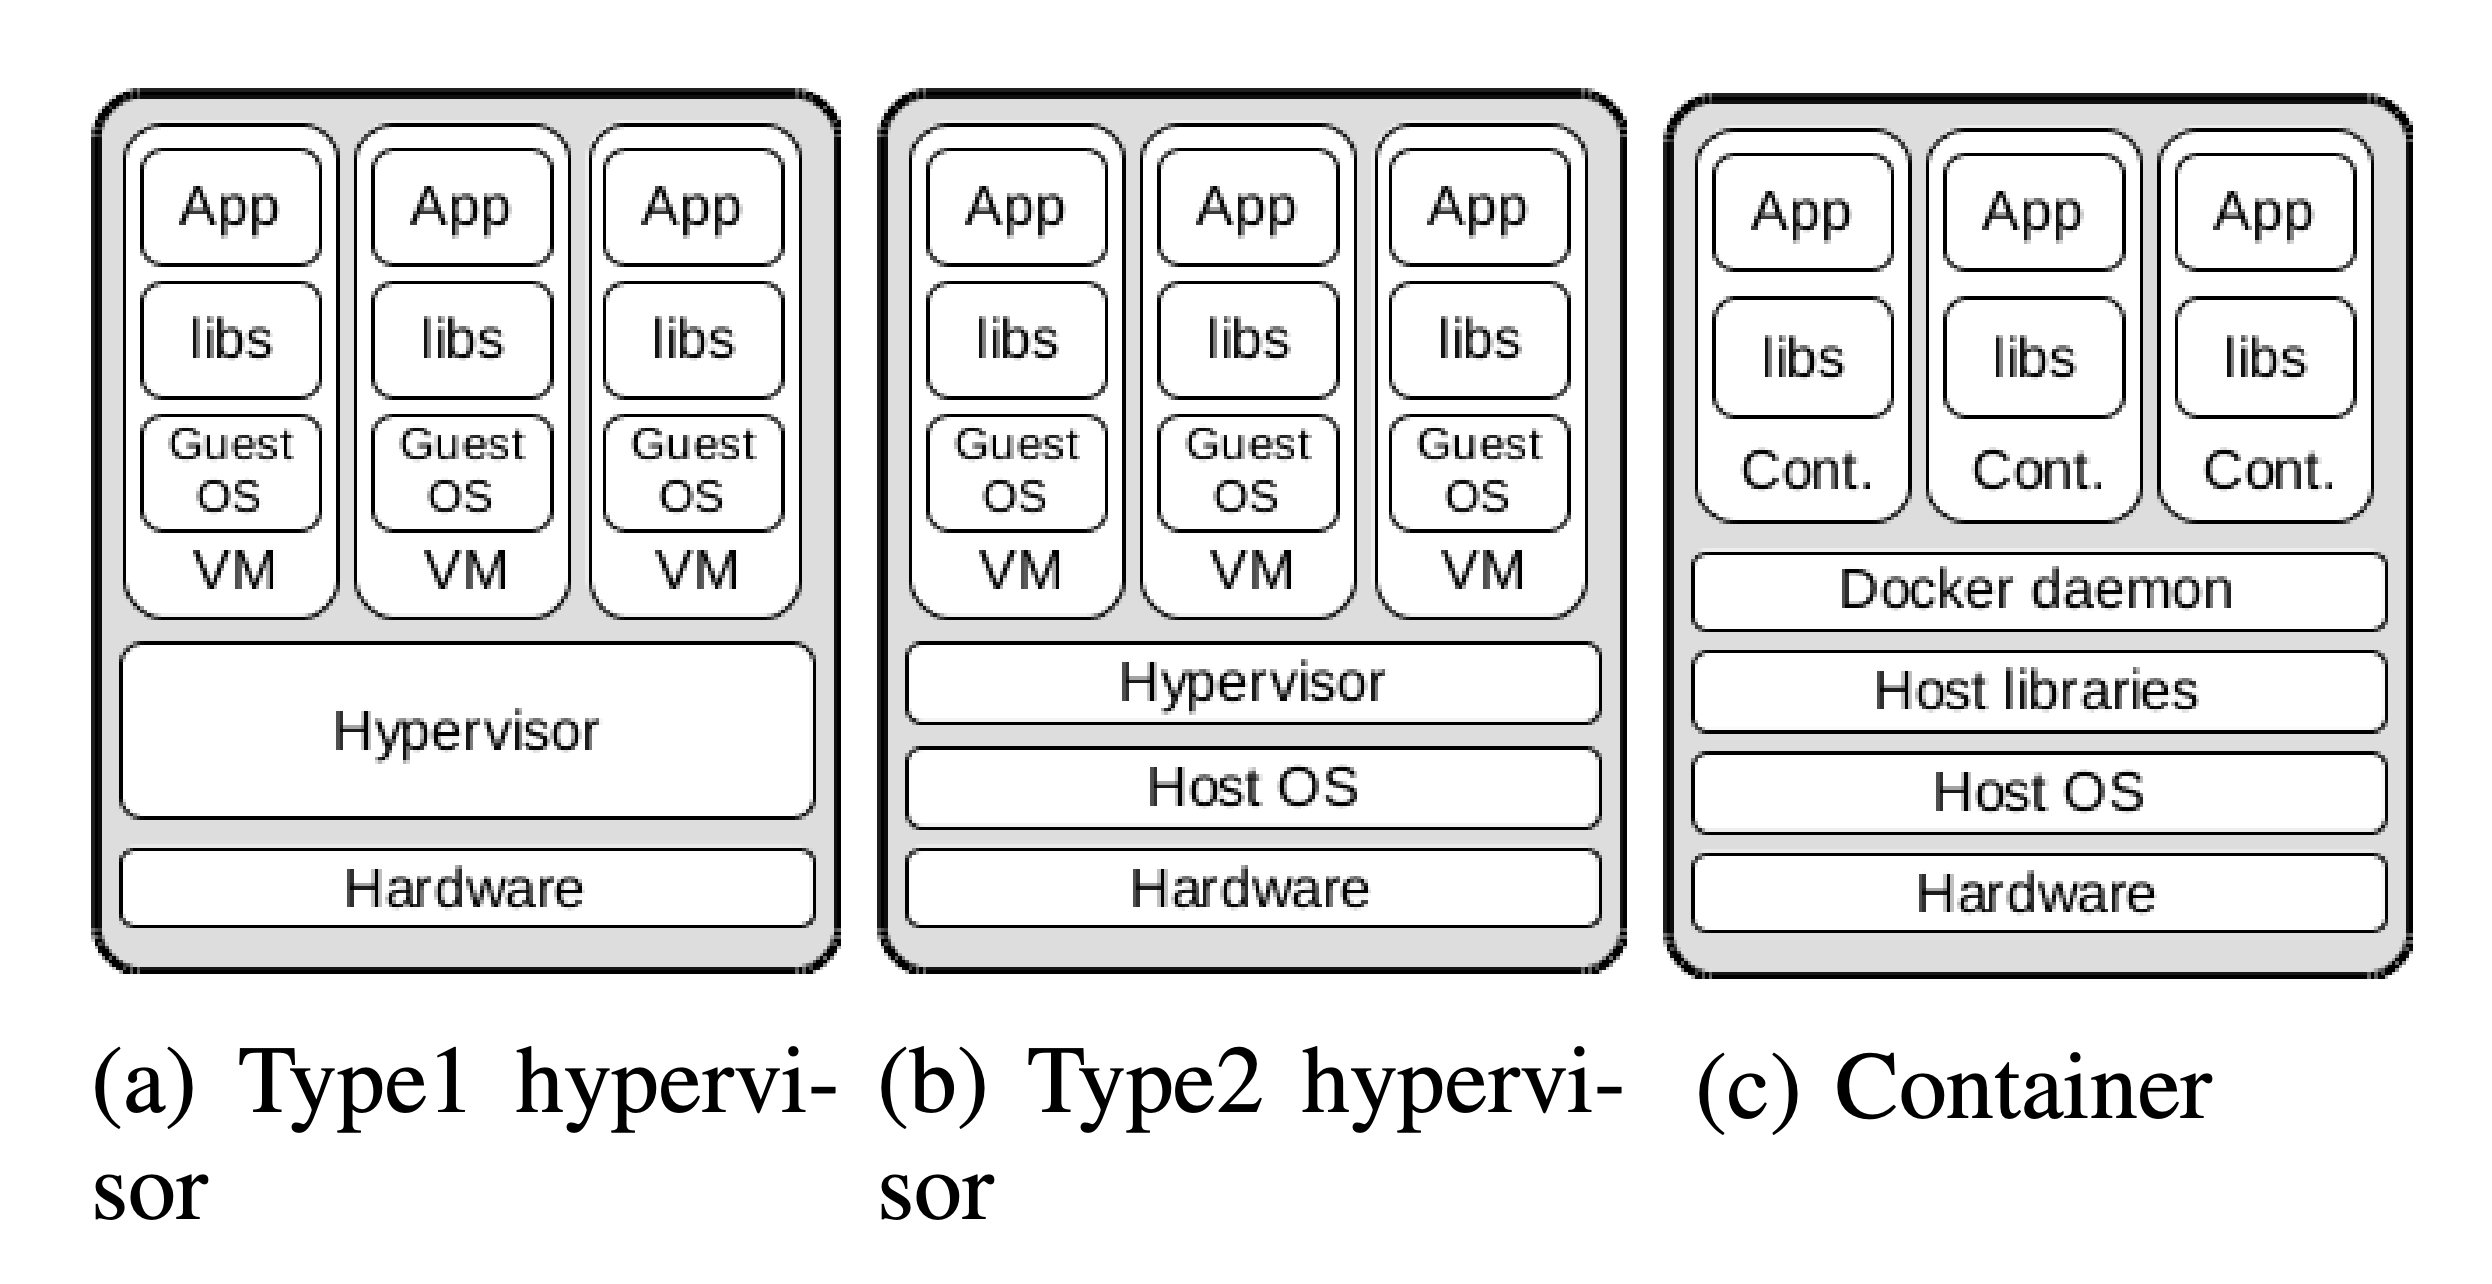
\includegraphics[width=\linewidth]{files/figure-1.png}
  \caption{Virtualization models \cite{combe2016docker}}
  \label{figure-1}
\end{figure}

Figure~\ref{figure-1} illustrates common virtualization models. Whereas traditional virtualization techniques virtualize workloads on top of a hypervisor which shares hardware resources between the virtual machines, containerization is a technique where virtualization happens on a operating system level \cite{merkel2014docker}. Processes executing in containers run on the host machine kernel. However, each container is isolated to its own network, process namespace and so on; two containers on the same host OS do not know that they share resources. Furthermore, containers are similarly isolated from accessing host OS resources.

BSD jails and \textit{chroot} can be considered early forms of containerization technology, so the idea of containers is not new \cite{combe2016docker}. Recent Linux container solutions rely on two main implementations: Linux Containers (LXC) -based solution that relies on kernel features such as control groups (cgroups) and namespaces, and a custom kernel and Linux distribution called Open Virtuozzo (OpenVZ). Docker \cite{docker} is a hugely popular container runtime that is based on LXC and provides an easy-to-use API and tooling for creating and managing containers. Docker also provides containerization for other OSes as well. However, in this thesis we focus only on the Linux implementation.

\subsubsection{Linux containers}

The Linux containers technology implements container isolation and containement using Linux kernel feature called namespaces \cite{lin2018measurement}. Namespaces \cite{manpages-namespace} are a construct that wraps a global system resource in an abstraction which makes it appear to the processes in the namespace that they have their own, isolated, instance of the global resource. There are total of eight namespaces: i) Cgroup which is used for resource management, ii) Inter-process communication (IPC) which isolates POSIX message queues etc., iii) Network which isolates network devices, stack ports etc., iv) Mount for file system isolation, v) Process ID (PID), vi) Time, vii) User for isolating user and group identifiers and viii) UTS which isolates hostnames and NIS domain names. For example, network namespace provides each container their own loopback device and even \texttt{iptables} rules. In another example, mount namespace makes sure that container has no visibility nor access to the host's or other container's file system. Compared to other namespaces that concern isolation of kernel data, cgroups focuses on limiting available system resources per namespace \cite{lin2018measurement}. Each namespace can be setup with their own limits on CPU and memory usage and available devices. Using Docker as an example, setting \textit{--cpu}, \textit{--memory} and \textit{--devices} options will limit available resources for the container.

% One critical security risk of the container mechanism is that all containers running on the same host share the same Linux kernel. If a process inside the container compromises the Linux kernel, the isolation provided by the container mechanism becomes invalid. Therefore, several Linux kernel security mechanisms are adopted to constrain the capability of the processes inside the containers, such as Capability [48], Seccomp [29] and Mandatory Access Control (MAC) mechanisms. Through Capability mechanism, the superuser privilege (i.e., ROOT privilege) is divided into 38 distinct units, known as capabilities. Each capability represents a permission to process some speci"c kernel resources. For example, the CAP_NET_ADMIN capability denotes the permissions to perform network-related operations. By default, the containers created by Docker own 14 capabilities [21]. The Seccomp mechanism constrains the system calls a process can invoke. Docker de"nes the available system calls for a container through a Seccomp pro"le "le, which by default includes more than 300 system calls [26]. Both Capability and Seccomp are Discretionary Access Control (DAC) mechanisms, and SELinux [52] and AppArmor [24] are two MAC mechanisms adopted by containers. SELinux has been integrated in CentOS / RHEL / Fedora distros, and AppArmor has been integrated in Debian/Ubuntu distros. AppArmor utilizes a path-based enforcement model [5], while SELinux adopts a label-based enforcement model [52].

Since all containers and the host machine run on same kernel, any container that manages to breakout from isolation may compromise other containers, the host and the whole kernel. To combat this container breakout, several Linux kernel security mechanisms are adopted to constrain the capabilities of containers \cite{lin2018measurement}. The mechanisms include Discretionary Access Control (DAC) mechanisms like Capability \cite{manpages-capabilities} and Secure computing mode (Seccomp) \cite{manpages-seccomp}, and Mandatory Access Control (MAC) mechanisms like Security-Enhanced Linux (SELinux) and AppArmor \cite{apparmor}. With Capability, the superuser (i.e. the root user) privilege is divided into distinct units, each of which represent a permission to process some specific kernel resources. The feature turns the binary "root/non-root" security mechanism into fine-grained access control system, which makes it easier to follow the principle of least privilege. For example, processes like web servers that just need to bind on a Internet domain privileged port (numbers below 1024) do not need to run as root; they can just be granted with \texttt{CAP\_NET\_BIND\_SERVICE} capability instead \cite{docker-security}. The Seccomp mechanism constrains which system calls a process can invoke. The available system calls are defined for a container through Seccomp profile which is defined as a JSON file. The Docker default Seccomp profile \cite{docker-default-seccomp} includes over 300 system calls. SELinux is integrated to CentOS/RHEL/Fedora distributions and utilizes a label-based enforcement model, while AppArmor is available in Debian and Ubuntu distros and adopts a path-based enforcement model \cite{lin2018measurement}.

\subsubsection{Docker}

\begin{figure}[h!]
  \centering
  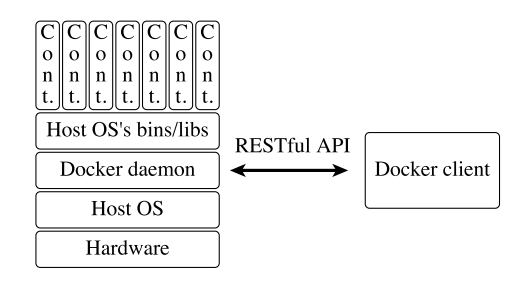
\includegraphics[width=\linewidth]{files/docker-engine.png}
  \caption{Architecture of Docker engine \cite{bui2015analysis}}
  \label{figure-docker}
\end{figure}

Docker is an open-source container technology written in Go and launched in 2013 \cite[text]{docker-what}. The platform consists of Docker Engine packaging tool, Docker image registries like the public image repository Docker Hub and Docker desktop application \cite{docker-overview}. In general, the engine architecture is similar to container-based virtualization, as visible in figure \ref{figure-docker} \cite{bui2015analysis}. The containers run on top of Docker daemon which manages and executes all the containers. The daemon is exposed to Docker clients via RESTful HTTP API. The Docker client is a command line tool which provides user interface for commanding the daemon and thus containers. By exposing the API outside the host machine, the architecture enables remote control of daemon with the client. For security reasons, remote communication should be secured with TLS.

Docker image is a read-only template with instructions for creating a Docker container \cite{docker-overview}. The images are often based on another image, such as OS images \texttt{ubuntu} and \texttt{alpine}, with some additional customizations like installation of web server binaries. The customizations are added to the image as series of data layers so that each new command creates a new layer. This process makes the distribution of image more efficient since only the changes between layers need to be distributed \cite{bui2015analysis}. The layering is achieved with special filesystem inspired by UnionFS which allows files and directories in different file systems to be combined into a single consistent file system.

Docker users can share their custom images publicly or privately in Docker Hub, or even host their own image registry platform. Most cloud providers also offer container registry services so even propietary software can be published in a private registry and used by other cloud services, like Kubernetes clusters. Whenever the image is not found locally, the client automatically tries to search and pull image from connected registries.

\subsection{Kubernetes}

Kubernetes (K8s) \cite{kubernetes} is an open-source container orchestrator, i.e. a system for automating deployment, scaling and management of containerized applications. It allows creation of a cluster which consists of a set of servers, called Nodes, on which application containers are scheduled by the system. The automation provides resilience and efficient resource utilization for workloads in the cluster: if a container or node dies, the system tries to restart and re-schedule containers so that the desired cluster state is maintained. K8s is hosted by the Cloud Nativce Computing Foundation (CNCF), but it's origins are at Google where it was created as an open-source option for Google's propietary Borg and Omega orchestrators \cite{burns2016borg}. K8s was open-sourced in 2014.

\subsubsection{Kubernetes objects}

\textbf{Pods} are the basic atomic scheduling unit in K8s. Pods consists of one or more tightly-coupled containers with shared storage volume and networking \cite{k8s-docs-pods}. Containers in a pod are always co-located and co-scheduled and run in a shared context, i.e. a set of Linux namespaces. Network, UTS and IPC namespaces are shared by default, and process namespace can be shared with \texttt{v1.PodSpec.shareProcessNamespace}. The common network namespace means that containers in a pod can communicate with each other via localhost, have common IP address and cannot re-use same port numbers. In addition to normal application container, Pods can include special \texttt{initContainers} that are only run on Pod startup. These pods are used for modifying Pod context before the actual workload starts. Multiple \texttt{initContainers} are run sequentially and a failing container blocks the execution of the following initialization and normal workloads. All Pods accross the cluster share same subnet and can access each other via IP address. However, connecting to a Pod with IP address is sub-optimal since Pods are ephermal and restarting a dead pod may receive a new IP address. Furthermore, horizontally scaled Pods with multiple replicas have as many IP addresses, thus making load balancing difficult. Kubernetes concept called Services solves these issues.

Instead of creating Pods directly, \textbf{Deployment} workload resources are used for creating Pods in a cluster, even with singleton Pods \cite{k8s-docs-pods}. With Deployments, user describes the desired state in a declarative manner. The Kubernetes control loop then creates \textbf{ReplicaSet} based on the Deployment resource, which in turn guarantees the availibility of desired amount of Pods \cite{k8s-docs-deployment}. \textbf{DaemonSet} on the other hand is a workload resource that ensures all or some Nodes run a copy of a Pod. Typical usecases for daemons are running Node monitoring and logging, and network plugins which was discuss in depth in section \ref{cni}.

\textbf{Services} are an object for exposing groups of Pods over an network \cite{k8s-docs-services}. The object defines a set of enpoints, i.e. the targeted pods, along with a policy about how to make the pods accessible. The targeted pods are determined with a \texttt{selector} field in the object specification. Meanwhile, the \texttt{type} field determines how the Service is exposed. There are four different \texttt{ServiceTypes} levels: i) the default \texttt{ClusterIP} which exposes Service inside the cluster with its own IP address, ii) \texttt{NodePort} which exposes service in each Node's IP address on static port (by default within a range of 30000-32767), iii) \texttt{LoadBalancer} which exposes the Service externally using cloud provider's load balancer and iv) \texttt{ExternalName} which is used to map Service to DNS name instead of a group of Pods. The field is designed as a nested functionality; each \texttt{ServiceType} level adds up to the previous one. Ingress object can also be used for exposing Services to outside of cluster. The Ingress object requires installation of an Ingress Controller to the cluster. Cloud providers often have their own controllers and all the examples in this thesis are executed on a local cluster where no external access is needed. Thus, the controllers are left as an exercise for the reader.

\textbf{Namespaces} provide isolation for cluster objects and allow grouping of objects under a single name. New K8s cluster starts with four namespaces: \texttt{default}, \texttt{kube-node-lease}, \texttt{kube-public} and \texttt{kube-system}. Namespaced objects like Deployments, Services and Pods are always deployed under a namespace which is \texttt{default} if not explicitly defined. \texttt{kube-system} is the namespace for all objects created by the K8s system which is discussed more in depth in the next section \ref{control-plane}. Namespaces also provide a scope for naming; names of resources need to be unique within a namespace, but not across namespaces. Namespaces are also used to enforce resource quotas, access control, and isolation for cluster users, for example in multi-tenancy setups. Pod Security Standards \cite{k8s-docs-pss}, which are used by Pod Security admission controller, are also defined at namespace level. Admission controllers are discussed in section \ref{admission-controllers}.

\subsubsection{Kubernetes components} \label{control-plane}

\begin{figure}[h!]
  \centering
  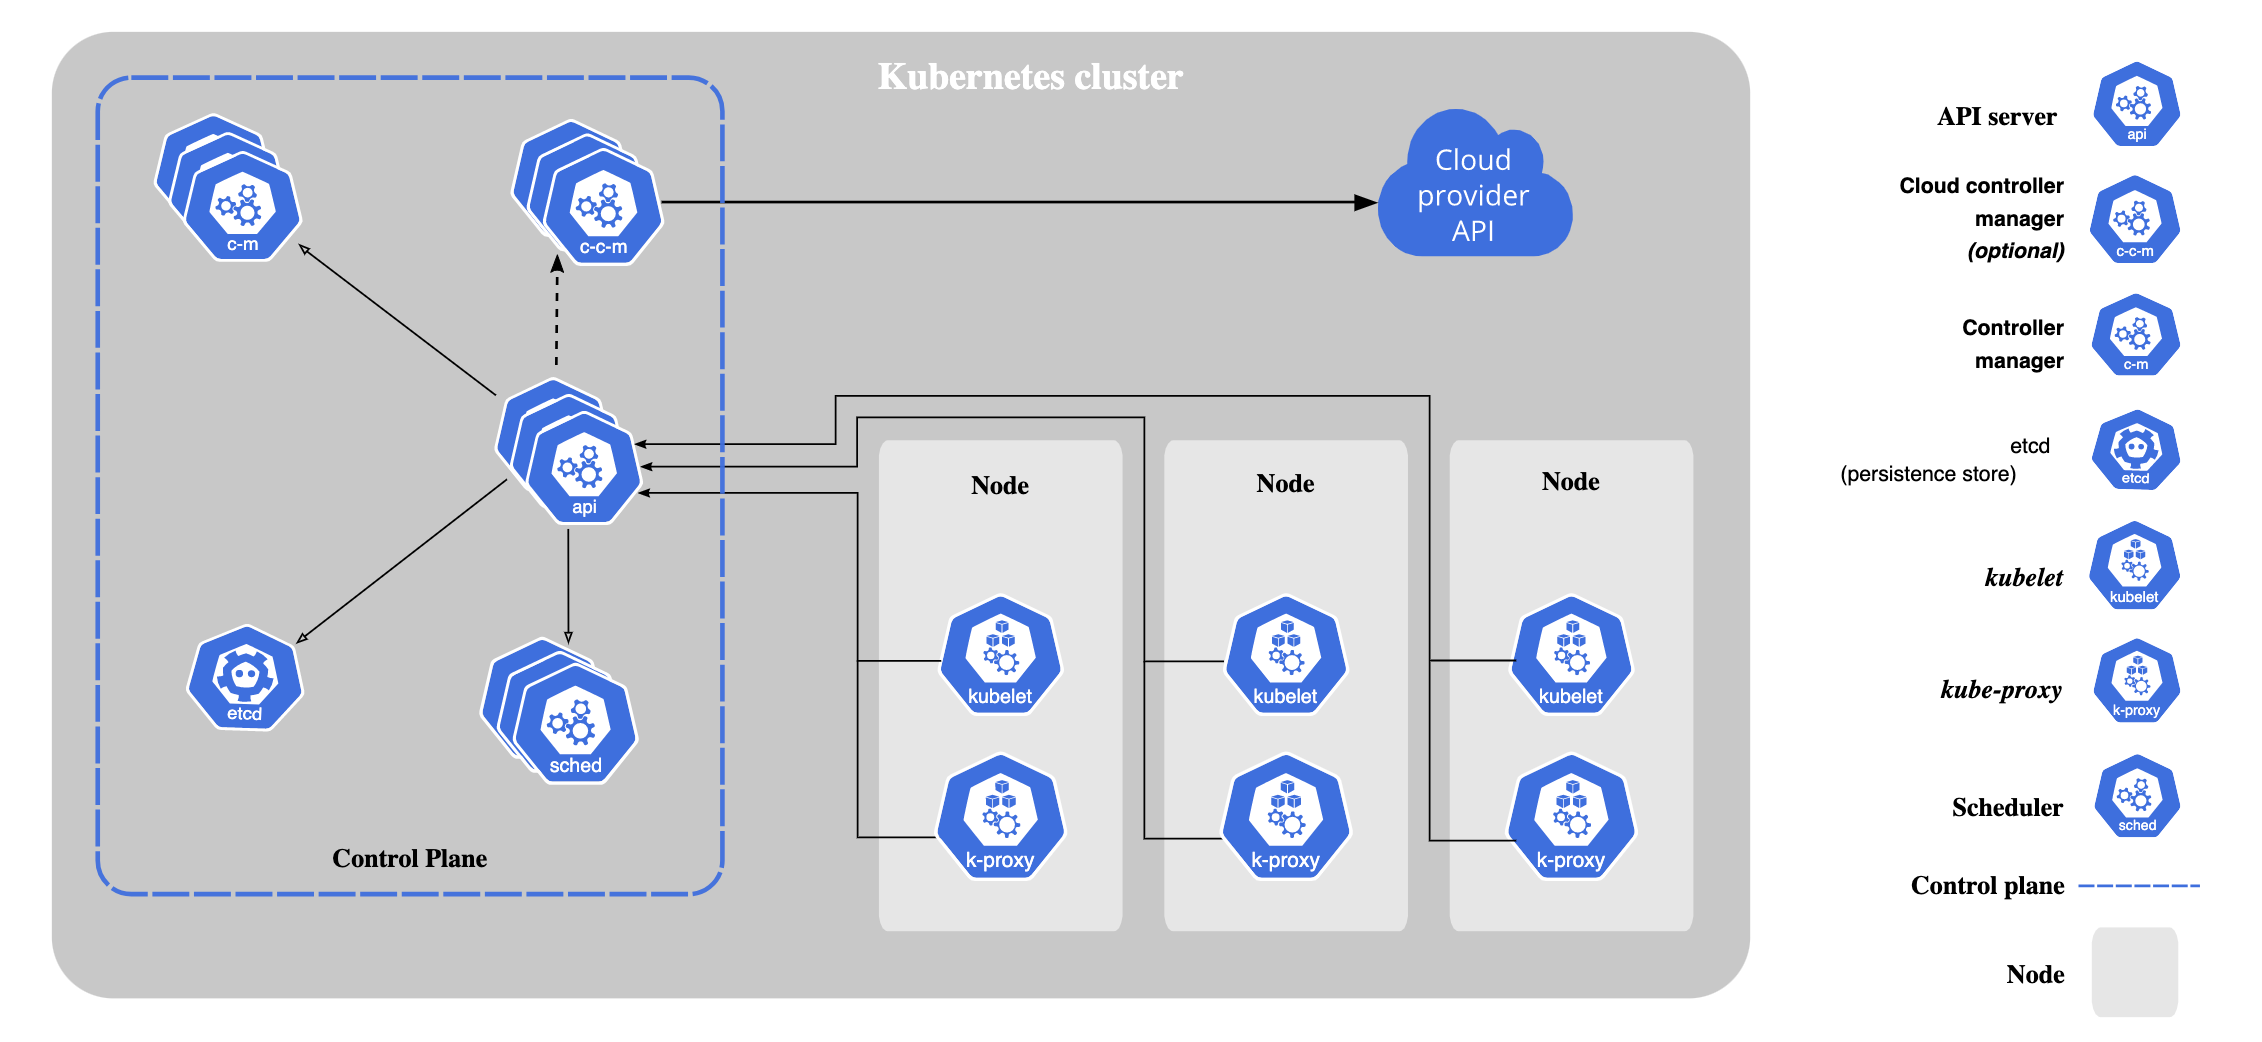
\includegraphics[width=\linewidth]{files/k8s-arch.png}
  \caption{Kubernetes cluster architecture \cite{k8s-docs-control-plane}}
  \label{figure-2}
\end{figure}

The figure \ref{figure-2} describes Kubernetes cluster with control plane and three worker nodes. The control plane consists of components that control, monitor and store the state of the cluster; essentially these are the components that are needed for complete and working Kubernetes cluster \cite{k8s-docs-control-plane}. The control plane components can be run on any worker node. However, clusters often have specialized master node for control plane components, which does not run any other containers. For fault-tolerance and high availability, control plane components should run on multiple Nodes in production environments. The control plane consists of these main components:

\textbf{API server} is a frontend component of the control plane. It is a stateless HTTP server which validates and authenticates commands given to the cluster. For valid commands, the server then forwards these to other control plane components. For example the \texttt{kubectl} CLI tool sends commands to the API server with HTTP. The main implementation of the server is \texttt{kube-apiserver}. The server can be horizontally scaled by running several instances on multiple Nodes and load balancing traffic between the instances.

\textbf{Etcd} \cite{etcd} is a strongly consistent, distributed key-value store. It is the stateful component of the control plane: all of the cluster data is stored in etcd. Thus, the stability of the component is critical for the whole cluster. To tolerate failures, etcd implements a leader-based architecture. Multiple etcd clients automaitcally elect a leader instance as the source of truth. Other instances periodically update their state from the leader instance, so that the state stays eventually conistent across all the instances. On leader failure, the other instances automatically elect new leader to keep the system functioning.

\textbf{Scheduler} watches for newly created Pods that have no assigned worker node, and selects one of the active Nodes for them to run on \cite{k8s-docs-control-plane}. The scheduling takes into account resource availibility on Nodes, Pod resource requirements, object specification affinity rules and hardware, software and policy constraints, among others.

\textbf{Controller manager} is a control plane component that runs all the controller loop processes \cite{k8s-docs-control-plane}. Controller loops, like the Deployment controller, continously watch the current and desired cluster state. When the states differ, they send commands via the API server so that the cluster moves towards the desired state. All the built-in controllers are compiled into a single binary, even though the controllers are logically different processes.

Each Node also has components that are essential for Kubernetes to work properly. \textbf{Kubelet} is an agent that makes sure containers are running in a Pod \cite{k8s-docs-control-plane}. It receives a set of pod specification from the API server and ensures that containers are running on the Node, follow the pod specifications and are healthy. Any container which is not created by Kubernetes is not managed by \texttt{kubelet}. \textbf{Kube-proxy} maintains network rules on Nodes. Part of the Serivce objects' networking is implemented by \textbf{kube-proxy}; the proxy writes \texttt{iptables} rules that route the traffic \cite{cilium-proxy-free}.

\subsubsection{Admission controllers} \label{admission-controllers}

Admission controllers are a feature of Kubernetes API server, made for  validating and modifying requests made to the server \cite{k8s-docs-admission}. The controllers execute prior to persistence of the object, but after the request is authenticated and authorized by the server. Several important features of Kubernetes are implemented with admission controllers, and these should be enabled in a properly configured API server. In addition to the built-in controllers, Kubernetes provides \texttt{MutatingAdmissionWebhook} and \texttt{ValidatingAdmissionWebhook} controllers for building own admission logic.

Admission controllers can be validating, mutating, or both \cite{k8s-docs-admission}. Mutating controllers may modify related objects to the requests they admit, while validating controllers either approve or reject the request. The control process executes mutating controllers first so that no mutations happen after the validation. If a controller in either phase rejects the request, the request is not processed further and error is returned to the end-user.

The important Admission controller for the scope of this thesis is the \texttt{PodSecurity} controller. The admission controller validates Pods before they are admitted, making sure that the requested Pod security context and other restrictions are permitted in the namespace that the Pod is assigned to \cite{k8s-docs-admission}. The controller is enabled by default, and can be taken into use just by configuring Pod Security Admission labels for Namespace objects.

The labels use \texttt{pod-security.kubernetes.io/<MODE>: <LEVEL>} format, where MODE defines the action to be taken when the security level is violated and the LEVEL is a pre-defined Pod Security Standard level. The three available levels are \texttt{privileged}, \texttt{baseline} and \texttt{restricted} \cite{k8s-docs-pss}.

The actions available are i) \texttt{enforce}, which will reject the pod on violation, ii) \texttt{audit}, which triggers an event about the violation in the audit log, and iii) \texttt{warn}, which triggers user-facing warning about the violation \cite{k8s-docs-psa}. A namespace can configure any or all three of the available modes, and even set a different level for the modes. For example, it is possible to warn the user about security policy violation without blocking the request by setting the \texttt{warn} mode more restrictive than the \texttt{enforce}.

% https://learn.microsoft.com/en-us/azure/architecture/patterns/sidecar
\subsubsection{Sidecar pattern}

As mentioned before, Pods are the basic scheduling abstraction in Kubernetes and they support management and co-scheduling of multiple containers as an atomic unit. This co-scheduling and management of multiple symbiotic containers as a single unit enables multi-container application design patterns to emerge \cite{burns2016design}. Sidecar pattern is the most common of these design patterns. As an example of this pattern, the main application container can be a simple web server pairted with a container that collects server's log file and streams them to a centralized log management system. Another example of this pattern is Istio service mesh \cite{istio} and its Envoy proxy sidecar which routes all traffic thorugh the Istio control plane for management, observability and security reasons.

% First, the container is the unit of resource accounting and allocation, so for example a web server container’s cgroup can be configured so that it provides consistent lowlatency responses to queries, while the logsaver container is configured to scavenge spare CPU cycles when the web server is not busy. Second, the container is the unit of packaging, so separating serving and log saving into different containers makes it easy to divide responsibility for their development between two separate programming teams, and allows them to be tested independently as well as together. Third, the container is the unit of reuse, so sidecar containers can be paired with numerous different “main” containers (e.g. a log saver container could be used with any component that produces logs). Fourth, the container provides a failure containment boundary, making it possible for the overall system to degrade gracefully (for example, the web server can continue serving even if the log saver has failed). Lastly, the container is the unit of deployment, which allows each piece of functionality to be upgraded and, when necessary, rolled back, independently. (Though it should be noted that this last benefit also comes with a downside – the test matrix for the overall system must consider all of the container version combinations that might be seen in production, which can be large since sets of containers generally can’t be upgraded atomically. Of course while a monolithic application doesn’t have this issue, componentized systems are easier to test in some regards, since they are built from smaller units that can be independently tested.) Note that these five benefits apply to all of the container patterns we describe in the remainder of this paper.

In the pattern, peripheral tasks such as logging, configuration and observability are isolated from the main application into helper containers. These containers, sidecars, are tightly-coupled to the parent application container and should share the lifecycle of the parent. Even though the functionality of the sidecars could be build into the main container, there are benefits for using separate containers \cite{burns2016design}. The isolation allows tweaking of containers' cgroups so that CPU cycles can be prioritized for the main container. The isolation also provides failure containement boundary between the main and sidecar processes. Since container is also the unit of deployment, the sidecar containers could be developed, tested and deployed independently from one another. Sidecar containers can also be developed with different tools and dependencies, and in a way that they are re-usable with other application containers. However, this multiplies the amount of moving parts of the overall system, which increases the size of test matrix considering all of the container version combinations that might be seen in the production environment.

\subsection{Kubernetes network model}

% https://kubernetes.io/docs/concepts/services-networking/
% https://kubernetes.io/docs/concepts/extend-kubernetes/compute-storage-net/network-plugins/

% The key requirements of the Kubernetes network model include i) Pods are IP addressable and must be able to communicate with all other Pods (on the same or different host) without the need for network address translation (NAT), and ii) all the agents on a host (e.g., Kubelet) are able to communicate with all the Pods on that host. CNI plugins may differ in their architecture but meet the above network rules.

Integral part of Kubernetes cluster is how nodes and resources are networked together. Specifically, the networking model needs to address four different type of networking problems: i) intra-Pod (ie. container-to-container within same Pod) communication, ii) inter-Pod communication between Pods, iii) Service-to-Pod communication and iv) communication from external sources to Services \cite{k8s-docs-cluster-networking}. The model also requires that each Pod is IP addressable and can communicate with other Pods without network address translation (NAT), even when Pods are scheduled on different hosts \cite{qi2020assessing}. All agents on a host should also be able to communicate with Pods on the same host. The implementation of this model is not part of Kubernetes, but is handed to special plugins that implement Container Network Interface (CNI) specification.

\subsubsection{Container Network Interface} \label{cni}

The Container Network Interface (CNI) \cite{cni} is a networking specification, which has become de facto industry standard for container networking. It is backed by CNCF \cite{qi2020assessing}. CNI was first developed for the container runtime \texttt{rkt}, but it is supported by all container runtimes and there is a large number of implementations to choose from \cite{hausenblas2018container}. Most of the container orchestrators have adopted the specification as their networking solution. The biggest outlier is Docker Swarm, which instead implements \texttt{libnetwork} \cite{libnetwork}.

The CNI specification has five distinct definitions: i) a format for network configuration, ii) a execution protocol between the container runtimes and the plugin binary, iii) a procedure for the runtime to interpret the configuration and execute the plugins, iv) a procedure for deletegating functionality between the plugins and v) data types for plugins to return their results to the runtime \cite{cni}. The network configuration is defined as a JSON file and it includes a list of plugins and their configuration. The container runtime interprets the configuration file at plugin execution time and transforms it into a form to be passed to the plugins. The execution protocol defines a set of operations (ADD, DEL, CHECK, VERSION) for adding and removing containers from the network. The operation command, similarly to other protocol parameters, are passed to the plugins via OS environment variables. The configuration file is supplied to the plugin via stdin. On successful execution, the plugin returns the result via stdout with a return code of 0. On errors, the plugin returns a specific JSON structure error message to stderr and a non-zero return code. When the runtime mutates a container network, it results in a series of ADD, DELETE or CHECK executions. These are then executed in same order as defined in the \texttt{plugins} list, or reversed order for DELETE executions. Each plugin then returns either \texttt{Success} or \texttt{Error} JSON object. The execution of a series of operations ends when it encounters the first Error response, or when all the operations have been performed.

% When a new Pod is added, the CNI plugin coordinates with the container runtime and connects the container network namespace with the host network namespace (e.g., , veth pair), assigns a unique IP address to the new Pod, applies the desired network policies and distributes routing information to the rest of the cluster.

% https://www.tkng.io/cni/

% Connectivity - making sure that a Pod gets its default eth0 interface with IP reachable from the root network namespace of the hosting Node.
% Reachability - making sure that Pods from other Nodes can reach each other directly (without NAT).

% Connectivity requirement is the most straight-forward one to understand – every Pod must have a NIC to communicate with anything outside of its own network namespace. Some local processes on the Node (e.g. kubelet) need to reach PodIP from the root network namespace (e.g. to perform health and readiness checks), hence the root NS connectivity requirement.

% Reachability, on the other hand, may require a bit of unpacking:
% - Every Pod gets a unique IP from a PodCIDR range configured on the Node.
% - This range is assigned to the Node during kubelet bootstrapping phase.
% - Nodes are not aware of PodCIDRs assigned to other Nodes, allocations are normally managed by the controller-manager based on the --cluster-cidr configuration flag.
% - Depending on the type of underlying connectivity, establishing end-to-end reachability between PodCIDRs may require different methods:
%   - If all Nodes are in the same Layer2 domain, the connectivity can be established by configuring a full mesh of static routes on all Nodes with NextHop set to the internal IP of the peer Nodes.
%   - If some Nodes are in different Layer2 domains, the connectivity can be established with either:
%     - Orchestrating the underlay – usually done with BGP for on-prem or some form of dynamically-provisioned static routes for public cloud environments.
%     - Encapsulating in the overlay – VXLAN is still the most popular encap type.

The CNI plugin must provide at least connectivity and reachability for the containers \cite{cni-tkng}. For connectivity, each Pod must have a NIC for communication outside its networking namespace. The NIC must have IP address reachable from the host Node, so that cluster processes like Kubelet health and readiness checks can reach the Pod. Reachability means that all Pods can be reached from other Nodes directly without NAT. Thus, each Pod receives an unique IP address from the \texttt{PodCIDR} range configured on the Node by the Kubelet bootstrapping phase. The end-to-end reachability between different Node \texttt{PodCIDR}s is established by encapsulating in the overlay network (for example with VXLAN) or orchestrating on the underlay network, e.g. with Border Gateway Protocol (BGP).

% Kubernetes Network Policy is the means to enforce rules
% indicating which network traffic is allowed and which Pods
% can communicate with each other. The policies applied to Pod
% network traffic can be based on their applicability to ingress
% traffic (entering the Pod) and egress traffic (outgoing traffic).
% The control strategies include “allow” and “deny”. By default,
% a Pod is in a non-isolated state. Once a network policy is
% applied to a Pod, all traffic that is not explicitly allowed will
% be rejected by the network policy. However, other Pods that do
% not have network policies applied to them are not affected. CNI
% plugins in Kubernetes can implement elaborate traffic control
% and isolation mechanisms.

% Network policies help to provide the guardrails needed to
% restrict traffic between pods (in and/or across namepaces) as
% well as between pods and external networks, by explicitly
% specifying allowed and denied connections. A network policy
% specification consists of a podSelector to specify pods
% that will be subject to the policy and policyTypes to
% specify the types of policies, i.e., ingress and/or egress. Ingress
% rules specify allowed inbound traffic to the target pods, and
% egress rules specify allowed outbound traffic from the target
% pods. Each rule is comprised of a NetworkPolicyPeer
% for selecting pods on the other side of the connection to/from
% which traffic is allowed, through a Classless Inter-Domain
% Routing (CIDR) notation that specifies IP address blocks,
% namespaces, or pod labels; and a NetworkPolicyPort
% that allows to explicitly specify ports or protocols that may
% communicate with the pod. Network policies are additive, and
% if multiple policies select a pod, traffic is restricted to what is
% allowed by the union of those policies’ ingress/egress rules.

Since Kubernetes does not provide networking between the Pods, it has no capabilities to enforce network isolation between workloads. Thus, another key feature for CNI plugins is enforcing network traffic rules. Kubernetes provides a common object called \texttt{NetworkPolicy} for CNI plugins to consume. The NetworkPolicy specification consists of a \texttt{podSelector} that specifies pods that are subject to the policy and \texttt{policyTypes} to specify Ingress and Egress rules for the traffic \cite{budigiri2021network} to the target Pod. Each rule includes \texttt{to} or \texttt{from} field for selecting Pod, Namespace or IP address block in CIDR notation on the other side of the connection, and \texttt{ports} field for explicitly specifying which ports and protocols are part of the rule. The policies are additive; when multiple rules are defined for a Pod, the traffic is restricted to what is allowed by the union of the policies. Many CNI plugins also introduce Custom Resource Definitions for their own, more granular, network policy rules.

While all CNI plugins meet the requirements listed above, they may differ in architecture significantly. The plugins can be classified based on which OSI model network layers they operate on, which Linux kernel features they use for packet filtering and which encapsulation and routing model they support for inter-host and intra-host communication between Pods. In this thesis, we focus on three different CNI plugins: Calico, Cilium and Multus.

% TODO: CNI plugins, daemons and binary \cite{qi2020understanding}.

% Src: https://www.youtube.com/watch?v=0jJBUdYOmRU
% Configurations in /etc/cni/net.d on nodes
% Kubelet monitors the directory, no need to restart it when installing CNI

\subsubsection{Calico}

Calico \cite{calico} is an open-source CNI plugin with modular architecture that supports wide range of deployment options. Each Pod created to the Calico network receives one end of a virtual ethernet device link as its default \texttt{eth0} network interface, while other end is left dangling on the host Node \cite{calico-tkng}. The Pod end of the link receives IP address from Pod CIDR, but the Node end does not. Instead, a \texttt{proxy\_arp} flag is set on the on the host side of the interface while containers have a route to link-local address \texttt{169.254.1.1}, thus making the host behave like a gateway router. For routing packets between Nodes, Calico creates a VXLAN overlay network. Optionally, Calico supports IP-in-IP overlay or non-overlay network with BGP protocol.

On each Node, a \texttt{calico-node} daemon setups CNI plugin, IPAM and possible eBPF programs. The daemon subscribes to Kubernetes API for Pod events and manages both container and host networking namespaces. Calico also deploys a single-container \texttt{calico-kube-controllers} Pod into the Kubernetes control plane. The container executes a binary that consists of controller loops for Namespace, NetworkPolicy, Node, Pod and ServiceAccount Kubernetes objects. The Calico project also introduces own CLI tool, called \texttt{calicoctl} \cite{calicoctl}, for managing Calico's custom resources. The tool provides extra validation for the resources which is not possible with \texttt{kubectl}.

Calico supports Kubernetes NetworkPolicies as well as its own namespaced \\\texttt{projectcalico.org/v3.NetworkPolicy} Custom Resource Definition (CRD). Both of the policies work on OSI layers L3 (identity, e.g. IP address) and L4 (ports). Compared to the built-in policy, the Calico policy includes features such as policy ordering, log action in rules, more flexible matching criteria (e.g., mathcing on ServiceAccounts) \cite{calico-network-policy}. The policy can also match on other Calico CRDs such as \textbf{HostEndpoints} and \textbf{NetworkSets}, which allows implementing rules on host interfaces and non-Kubernetes resources. If Calico is installed along Istio service mesh, the Calico Network Policy can enforce L7 (e.g. HTTP methods and URL paths) policies on the Envoy proxy. For policies that are not tied to a Kubernetes namespace, Calico provides a \texttt{GlobalNetworkPolicy} CRD.

\subsubsection{Cilium}

Cilium \cite{cilium} is one of the most advanced and powerful CNI plugins for Kubernetes. Similarly to Calico, it creates virtual ethernet device for each Pod and sets one side of the link into Pod's network namespace \cite{cilium-tkng} as the default interface. Cilium then attaches extended Berkeley Packet Filter (eBPF) programs to ingress traffic control (\texttt{tc}) hooks of these virtual ethernet devices for intercepting all incoming packets from the Pod. The packets are intercepted and processed before the network stack and thus \texttt{iptables}, reducing latency 20\%-30\% and even doubling the throughput of packets in some scenarios \cite{budigiri2021network}. The network between Pods running on different hosts is handled by default with VXLAN overlay, but there is support for Geneve interfaces and native-routing with BGP protocol as well \cite{cilium}.

The Cilium system consists of an agent (\texttt{cilium-agent}) daemon running on each Node, one or more operator (\texttt{cilium-operator}) Pods and a CLI client (\texttt{cilium}) \cite{cilium-components}. The agent daemons subscribe to events from Kubernetes API and manage containers' networking and eBPF programs. The CLI tool, which is installed on each agent, interacts with the REST API of the agent and allows inspecting the state and status of the local agent. The tool should not be confused with Cilium management CLI tool, also incidentally named \texttt{cilium}, which is typically installed remote from the cluster. The operator is responsible for all management operations which should be handled once for the entire cluster, rather than once for each Node. This includes for example registering of CRDs.

% TODO: Move OSI layer to somewhere else
While default Kubernetes Network Policy provides security on OSI layers L3 and L4, Cilium provides CRDs that also support for L7 policies \cite{cilium-policy-language}. If L7 policies exist, the traffic is directed to Envoy instance bundled into the agent Pod which filters the traffic. Unlike on layers 3 and 4, policy violation does not result in dropped packet but an application protocol specific denied message. For example, HTTP traffic is denied with \texttt{HTTP 403 Forbidden} and DNS requests with \texttt{DNS REFUSED}. Cilium provides \texttt{CiliumNetworkPolicy} CRD that supports all L3, L4 and L7 policies. Cilium also provides \texttt{CiliumClusterwideNetworkPolicy} custom resource which is used to apply network rules to every namespace in the cluster or even to nodes when using \texttt{nodeSelector}.

As even more advanced features, Cilium also includes natively \texttt{kube-proxy} replacement, encryption for Cilium-managed traffic and Service Mesh, among others. By default, \texttt{kube-proxy} uses \texttt{iptables} to route the Service traffic \cite{cilium-proxy-free}. With \texttt{kubeProxyReplacement} installation option, Cilium implements Service load-balancing as XDP and TC programs on Node network stack. For encryption, Cilium supports both IPsec and WireGuard implementations \cite{cilium-encryption}. The Service mesh performs variety of features directly in eBPF, thus functioning without sidecar containers or proxying requests through the agent Pod's Envoy \cite{cilium-service-mesh}. Since all features are not available as eBPF programs or on all kernel versions,  Cilium automatically probes the underlying kernel and automatically reverts to Envoy proxy when needed. For capabilities beyong the built-in mesh, Cilium also provides an integration with Istio.

% \begin{itemize}
  % \item More on network rules (probes and uses most recent features from Kernel)
  % \item Transparent encryption https://docs.cilium.io/en/v1.13/security/threat-model/
  % \item Security on different levels: https://docs.cilium.io/en/v1.13/security/network/intro/
  % \item Cilium Service Mesh https://isovalent.com/blog/post/cilium-service-mesh/
  % \item Kube-proxy replacement
  % \item Cilium components (Agent (includes Envoy), client, operator, plugin). Hubble?
% \end{itemize}

\subsubsection{Multus}

Traditionally CNI plugins only provide a single network interface for a Pod, apart from loopback device. Multus \cite{multus-cni} is a CNI plugin that allows attaching multiple network interfaces for a Pod. It does not provide any connectivity or reachability for the containers like other plugins. Instead, it is installed as the first plugin in the CNI plugin chain. When executed, the plugin delegates interface creation to other installed plugins. Since Multus does not provide any networking and thus does not independently, it is often called "meta plugin" to distinguish it from common CNI plugins like the previous Calico and Cilium.

Multus system includes a binary, a CNI configuration file and a namespaced \texttt{NetworkAttachmentDefinition} CRD that is used to define network interfaces used in Pods. The binary and the configuration file are often installed to cluster Nodes via a DaemonSet. The daemon consists of an \textit{initContainer} that copies the binary into the \texttt{/opt/cni/bin} directory, and a daemon container that setups the configuration file and optionally spawns a HTTP server for additional features such as metrics \cite{multus-cni}. The configuration file satisfies the CNI specification with few extra attributes of which the combination of \texttt{clusterNetwork} and \texttt{defaultNetworks} or \texttt{delegates} are imperative for the CNI plugin to function \cite{multus-cni-config}. The \texttt{clusterNetwork} specifies the main network of the cluster, which implements the \texttt{eth0} interface and Pod IP address. The \texttt{defaultNetworks} is an optional array of networks that should be added for any Pods by default. The values can be names of the \texttt{NetworkAttachmentDefinition} objects or paths to CNI plugin's JSON configuration files. Optionally, the \texttt{delegates} attribute can be used; it supports similar format of values. In this scenario, the first element of the array functions as \texttt{clusterNetwork} and the rest are infered as \texttt{defaultNetworks}.

% TODO: Add examples of NetworkAttachmentDefinition and Pod annotations

Attaching additional interfaces to workloads is most often configured by adding a special annotations field \texttt{k8s.v1.cni.cncf.io/networks} to workload resource definitions. In the simplest configuration, the field takes a comma-separated list of \texttt{NetworkAttachmentDefinition} names as input. The network interface identifiers can be modified by giving the attachment input in \textit{name@interface-identifier} format. Otherwise, Multus names the interfaces \textit{net0}, \textit{net1} and so on. If extra configuration for the networks is needed, the annotation also supports a JSON array format.

\subsubsection{Extended Berkeley Packet Filter}

Berkeley Packet Filter (BPF, or nowadays often cBPF) was originally developed in early 1990s as a high-performance tool for user-space packet captures \cite{mccanne1993bsd}. BPF works by deploying the filtering part of the application, \texttt{packet filter}, in the kernel-space as an agent. The \texttt{packet filter} is provided with a program (often denoted as BPF program) consisting of BPF instructions, which works as a set of rules for selecting which packets are of interest in the user-space application and should be copied from kernel-space to user-space. The instuctions are executed in a register-based pseudo machine. Since network monitors are often interested only in subset of network traffic, this limits the number of expensive copy operations across the kernel/user-space protection boundary only to packets that are of interest in the user-space application. A notable usecase for BPF is \textit{libpcap} library, which is used by network monitoring tool called \texttt{tcpdump}.

Later in the 2010s the Linux community realized that BPF and it's ability to instrument the kernel could benefit other areas than packet filtering as well \cite{vieira2020fast}. This reworked version of BPF was first merged in to Linux kernel in 2014 and is publicly called extended Berkeley Packet Filter (eBPF) to distinguish it from the original cBPF. The kernel development community continues to call the newer version BPF, but instead of the original acronym consider it a name of a technology. Similarly to the kernel community, the term BPF always refers to the eBPF in this thesis.

The eBPF programs are compiled to bytecode and loaded to kernel with \texttt{bpf()} system call \cite{miano2021framework}. Most often programs are written in restricted C and compiled with LLVM Clang compiler to bytecode. It also possible to use eBPF assembly instructions and \texttt{bpf\_asm} utility for converting instructions to bytecode. eBPF programs follow a event-driven architecture: a loaded eBPF program is hooked to a particular type of event and each occurence of the event triggers the program execution.

% TODO: Yhidstä johonkin kappaleeseen
For networking purposes, there are two eBPF hooks available for intercepting and mangling, forwarding or dropping network packets: eXpress Data Path (XDP) and Traffic Control (TC) \cite{miano2021framework}. In Cloudflares DDoS testing benchmark \cite{cloudflare-xdp}, XDP program was capable to drop 10 million and TC program 2 million packets per second, while common \texttt{iptables} INPUT rule was able to drop less than one million packets per second.

XDP programs are attached to a network interface controller (NIC) and can handle only incoming packets \cite{hoiland2018express}. The programs are called directly by the NIC driver if it has XDP support, thus executing before packets enters the network stack. This skips expensive packet parsing and memory allocation operations, and allow XDP programs to run at very high throughput. Thus, even the main networking buffer \textit{skbuff} is not populated. Some SmartNICs even support offloading the program to the NIC's own processor from host CPU, improving host machine performance even further \cite{cilium-program-types}. If the driver does not support XDP, generic XDP is used and the programs run after the packet has been parsed by the network stack.

XDP programs can read and modify contents of the packets \cite{vieira2020fast}. Since the packets are not parsed the network stack, the programs have to work with raw packets and implement own parsing functionality. The program's return value determines how the packet should be processed further. With \texttt{XDP\_DROP} and \texttt{XDP\_PASS} return values, the packet can be dropped or passed further to the networking stack respectively. The packet can also be bounced back to the same NIC it arrived on with \texttt{XDP\_TX}, usually after modifying the packet contents. \texttt{XDP\_REDIRECT} is used for redirecting the packet to a different NIC, CPU or even to another socket.

TC programs are executed when both incoming and outgoing packets reach kernel traffic control function within the Linux network stack \cite{vieira2020fast}. The ingress hook executes after the packet is parsed to \textit{skbuff} but before most of the network stack. On egress the stack is traversed in reverse, thus the hook executes after most of the network stack. TC programs can read and write directly to packet in memory. Similarly to XDP programs, the return value of the program determines further processing of the packet. The packet can be passed furhter in the stack with \texttt{TC\_ACT\_OK}, dropped with \texttt{TC\_ACT\_SHOT}, or the modified packet can be redirected back to the start of the classification with \texttt{TC\_ACT\_RECLASSIFY}, among others.

\clearpage

\section{Research material and methods} \label{sec:methods}

This chapter analyzes threats in K8s cluster from the perspective of sidecars and defines security requirements for solution introduced in following chapters. First, threat modelling is used to identify possible attack vectors and readily available mitigations. Then, the model is used to identify all issues that should be solved with the solution. Finally, an example development envrionment is introduced for testing out the solution.

\subsection{Threat modelling}

\begin{table}[H]
  \centering
  \caption{Threat model}
  \label{table:threat-model}
  \sffamily% change the font in the table to sans serif
  \begin{tabularx}{\textwidth}{CCC}
    \hline
    \textbf{Threat} & \textbf{Description} & \textbf{Mitigation}\\ \hline
    Permissive container configurations & If containers are given privileges, malicious actor can breakout from the container and escalate the attack on cluster. & Use \texttt{restricted} Pod Security Admission to enforce security rules. Isolate privileged containers into own namespaces. \\ \hline
    Permissive RBAC on service accounts & By default, Pods automatically mount service account to all containers. & Set \texttt{automountServiceAccountToken: false} and explicitly mount SAs when necessary. \\ \hline
    No resource limits for containers & If no limits are set, single container can hog all available resources and affect availability of the service & Set resource limits to containers with \texttt{spec.containers[*].resources}. \\ \hline
    Pod is allowed to access access control plane components &  & Firewall Pods from \texttt{kube-system} namespace with NetworkPolicies. Explicitly add allow policy when needed. \\ \hline
    Sidecar can use main containers NetworkPolicy to access \texttt{kube-system} & NetworkPolicies affect Pod network devices. Sidecars share the device with the main container. & No built-in solution available! \\ \hline
    Sidecar has network access to main container & Containers in a Pod share NICs. Main container is accessible via loopback device. & No built-in solution available! \\ \hline
    Sidecar is used to sniff main application's traffic & TODO & TLS? \\ \hline
    Unencrypted secrets & TODO & Encrypt at rest \\ \hline
  \end{tabularx}
\end{table}

\clearpage

\section{Pod Privilege Escalation}

This chapter discusses securing K8s Pods from privilege escalation. First, possible attack scenarios are introduced and a solution for mitigating these issues is proposed. The solution itself sets some constraints on the network solution, which is discussed more in depth in the next chapter. As a baseline requirement, the networking solution should not enable sidecar container breakouts. Finally, some of the noted limitations of the solution are discussed.

\subsection{Example attack scenarios}

All of the example attack scenarios start by attacker getting shell access to a container running in a Pod, usually through a remote code exectuion (RCE) flaw on the container application and then executing reverse shell inside the Pod. The scope of the examples is not in the initial attack, but in the Pod template misconfiugrations that then provide some path for the attacker to escalate the attack and even take over the whole cluster in the end.

TODO: add file \label{yaml:priv-container}

The first attack scenario includes a privileged container, as described in file \ref{yaml:priv-container}. Privileged containers have all the capabilities of the host machine, so practically they can be perform almost any action available on the host. This includes but is not restricted to for example "pipeing" (TODO: better word for undock.sh and other scripts) commands as root to the Node's shell and mounting the host's disks. If combined with \texttt{hostPID:\ true}, the attacker can see all the processes on the host, and use \texttt{nsenter} to execute commands in the other processes' namespaces.

TODO: add file \label{yaml:host-path}

The second example file \ref{yaml:host-path} does not have similar privileges for executing commands as the first, but has unlimited access for mounting the whole host's filesystem, with both read and write access. Thus, the attacker can try to find any credentials stored on the host machine and use these to escalate the attack. Important credentials include \texttt{kubeconfig} files which store access token to K8s API server, ServiceAccount tokens that may have been mounted on any Pod on the host, SSH keys and hashed user passwords in \texttt{/etc/shadows}.

TODO: some extra issues (finding .kubeconfig files, running on control-plane -> etcd and secrets within, cloud metadata)

\subsection{Hardening containers}

For Kubernetes versions bigger than 1.25, the easiest way to enforce secure Pod configurations is to use Pod Security Admission controller, which was discussed in chapter \ref{admission-controllers}. The \texttt{restricted} Pod Security Standard aims on Pod hardening best practices \cite{k8s-docs-pss}, so it will be used in the solution. The table \ref{table:pod-hardening} describes all the fields affected by the standard.

\begin{table}[H]
  \centering
  \caption{Restricted security standard enforcement}
  \label{table:pod-hardening}
  \sffamily% change the font in the table to sans serif
  \begin{tabularx}{\textwidth}{CCC}
    \hline
    \textbf{Field name} & \textbf{Usage} & \textbf{Allowed values}\\ \hline
    hostPID, hostIPC, hostNetwork & Controls whether container uses host's PID, IPC and network namespace. & false \\ \hline
    privileged & Controls whether Pod can run privileged containers. & false \\ \hline
    capabilities.add & Defines Linux capabilities for the container. & NET\_BIND\_SERVICE \\ \hline
    capabilities.drop & Defines Linux capabilities for the container. & ALL \\ \hline
    volumes[*] & All volume types are not allowed. For example, hostPath, that maps host directories, are not allowed. & \texttt{volumes[*].configMap}, \texttt{volumes[*].csi}, \texttt{volumes[*].downwardAPI}, \texttt{volumes[*].emptyDir}, \texttt{volumes[*].ephemeral}, \texttt{volumes[*].persistentVolumeClaim}, \texttt{volumes[*].projected}, \texttt{volumes[*].secret} \\ \hline
    hostPort & Expose container via host's network port. & undefined \\ \hline
    container.apparmor.security.beta.kubernetes.io/* annotation & Sets the AppArmor profile used by containers.
    On supported hosts, the runtime/default AppArmor profile is applied by default. & runtime/default, localhost/* \\ \hline
    seLinuxOptions & Sets the SELinux context of the container. & Set if supported by environment. \\ \hline
    procMount & The default /proc masks are set up to reduce attack surface, and should be required. & Default \\ \hline
    seccompProfile.type & Sets the seccomp profile used to sandbox containers. & RuntimeDefault or Localhost \\ \hline
    sysctls[*].name & Sysctls can disable security mechanisms or affect all containers on a host, and should be disallowed except for an allowed "safe" subset. & kernel.shm\_rmid\_forced, net.ipv4.ip\_local\_port\_range, net.ipv4.ip\_unprivileged\_port\_start, net.ipv4.tcp\_syncookies, net.ipv4.ping\_group\_range \\ \hline
    allowPrivilegeEscalation & Restricts escalation to root privileges. & false \\ \hline
    runAsNonRoot & Controls whether container can run as root user. & true \\ \hline
    runAsUser, runAsGroup & Controls the user and group used by container. & Set both to non-zero to run as non-root. \\ \hline
    windowsOptions.hostProcess & Runs Windows containers as privileged HostProcess. & false \\ \hline
  \end{tabularx}
\end{table}

% resources & Sets resource limits for the container. & Add limits, containers without limits can starve other containers. \\ \hline
% readOnlyRootFilesystem & Requires the use of a read only root file system. & Set to true when possible. \\ \hline


% The table \ref{table:container-hardening} describes secuirty related fields in Pod templates \cite{nsa-cisa-hardening}.

% \begin{table}[H]
%   \centering
%   \caption{}
%   \label{table:container-hardening}
%   \sffamily% change the font in the table to sans serif
%   \begin{tabularx}{\textwidth}{CCC}
%     \hline
%     \textbf{Field name} & \textbf{Usage} & \textbf{Recommendation}\\ \hline
%     privileged & Controls whether Pod can run privileged containers. & Set to false. \\ \hline
%     hostPID, hostIPC, hostNetwork & Controls whether container uses host's PID, IPC and network namespace. & Set each to false. \\ \hline
%     % allowedHostPaths & Limits container to specific paths of the host file system. & Use a “dummy” path name (such as “/foo” marked as read-only). \\ \hline
%     readOnlyRootFilesystem & Requires the use of a read only root file system. & Set to true when possible. \\ \hline
%     runAsUser, runAsGroup & Controls the user and group used by container. & Set both to non-zero to run as non-root. \\ \hline
%     runAsNonRoot & Controls whether container can run as root user. & Set to true. Enforces above fields. \\ \hline
%     % This measure is required to effectively enforce “runAsUser: MustRunAsNonRoot” settings.
%     allowPrivilegeEscalation & Restricts escalation to root privileges. & Set to false. \\ \hline
%     seLinuxOptions & Sets the SELinux context of the container. & Set if supported by environment. \\ \hline
%     % AppArmor annotations & Sets the AppArmor profile used by containers. & Set if supported by environment. \\ \hline
%     seccompProfile & Sets the seccomp profile used to sandbox containers. & Enable a seccomp profile that blocks all unnecessary syscalls. \\ \hline
%     resources & Sets resource limits for the container. & Add limits, containers without limits can starve other containers. \\ \hline
%     capabilities & Defines Linux capabilities for the container. & Drop all capabilities, and enable just the ones required. \\ \hline
%   \end{tabularx}
% \end{table}

\cite{nsa-cisa-hardening}




\begin{itemize}
  \item Privileged container
  \item CAP\_SYS\_ADMIN, mounting /proc and chroot
  \item CAP\_SYS\_PTRACE, shellcode injection to running program, nc 172.17.0.1 on port running shell
  \item Mounted docker socket, creating privileged containers
\end{itemize}

\subsection{Pod Security Admission}

\subsection{Solution}

\clearpage

\section{Network Isolation}

\subsection{Requirements}

By Pod definition, all containers in a Pod share network namespace. The containers have common network interfaces, including loopback device, and thus a common IP address. For building a zero trust network model inside the namespace, the Pod must be firewalled for both inter-Pod communications from the Pod network interface and intra-Pod communications on the loopback device.

For inter-pod communications, the built-in NetworkPolicy is not sufficient since the source IP address in shared among all the containers. Furthermore, the intra-Pod communication on the loopback device also has the same source IP address of \texttt{127.0.0.1}, which is also the destination address. The pair of source IP address and source ephemeral port would be an unique identifier for the communication; however, this would require application layer implementation to reserve ports per container.

\subsection{IPTables}

One possible solution for firewalling sidecar from the application is using IPTables.

Usually IPTables rules only refer to IP addresses and ports. However, IPTables ships with an owner module, which support rules based on application's user, group, process (TODO: check this) and session identifier.

Running IPTables in Pod context requires root user permissions with NET\_ADMIN and NET\_RAW capabilities.

The execution context of

\begin{itemize}
  \item If executed from containers in Pod (init, lifecycle, wrapper container), it breaks Security admission rules (root user and NET\_ADMIN)
  \item Can be executed from Node itself, using DaemonSet (sort of a CNI plugin), but a bit hacky.
  \item Use owner module for catching egress packets (userId, groupId, processId)
\end{itemize}

\subsection{eBPF program firewall}

\begin{itemize}
  \item XDP works only for ingress
  \item TC needs some way to catch egress from sidecar
\end{itemize}

\subsection{Own pod for sidecar}

\begin{itemize}
  \item Guaranteed to work, since own network namespaces. What type of issues arise from this?
  \item Need to force pods to same node, for common volumes (if using host as storage)
  \item Implementation by hand, or Admission controller that catches sidecars?
  \item Loopback is not the same anymore. DNAT that changes localhost to external? => impossible with IPTables!
\end{itemize}

\subsection{Multus}

\begin{itemize}
  \item Requires breaking sidecar pattern with multiple Pods
  \item Allows use of custom IP addresses
  \item Hard to implement between nodes, affinity rules
  \item Loopback not easy to hijack for forwarding to new IPs
\end{itemize}

\clearpage

\section{Solution Evaluation} \label{sec:solution}

\clearpage

\section{Discussion} \label{sec:discussion}

\clearpage

\section{Conclusion} \label{sec:conclusion}

\clearpage

%% Bibliography/ list of references
\thesisbibliography
\printbibliography

%% Appendices
%% If you don't have appendices, your thesis ends here. Remove \clearpage, \thesisappendix and the following text below. The last command of this file is \end{document}.
\clearpage

\thesisappendix

\section{Contents of an appendix}
\label{app:contents}

Appendices are not essential in a thesis, and so you must plan the content of
your thesis as if it does not contain an appendix. The appendix cannot be used
as a dumping ground for text and ideas from an overgrown thesis.

An appendix is an independent entity, even though it complements the thesis.
So, the appendix is not, say, just a list or image or table, but contains
explanatory text as well that indicates the purpose of its content. It can
contain code listings, like the one below for a simplified list of commands to
create an appendix.
\begin{verbatim}
  \clearpage
  \appendix
  \addcontentsline{toc}{section}Contents of an appendix
  \thispagestyle{empty}
  \section*{Contents of an appendix}
  ...
  text
\end{verbatim}

Equation numbering in the appendix forms a separate, complete entity. Here are a couple of examples how equations in an appendix are numbered:
% \begin{align}
%   (x+a)^n &= \sum_{k=0}^n \binom{a}{b} x^n a^{n-k}, \label{appeq:1}\\
%   \sin\alpha \pm \sin\beta &= 2\sin\left(\frac{\alpha\pm\beta}{2}\right)
%   \sin\left(\frac{\alpha\mp\beta}{2}\right). \label{liitekaava2}
% \end{align}

% The appendix can contain figures that do not fit in to complement the text in
% the thesis. The numbering of figures is like that of equations: see figure~\ref{appfig:refraction}.

%% Example of a figure in the appendix. Note how b places the figure at the bottom of the page.
% \begin{figure}[b]
%   \centering
%     \includegraphics[height=31mm]{./linediagram.pdf}
%   \caption{Figure and caption to show the numbering in the appendix.}
%   \label{appfig:refraction}
% \end{figure}

% The numbering of tables is like that for equations and figures, as is evident
% from the caption of table~\ref{apptab:schedule}.

%% Example of a table in the appendix. Note how h places the table in the current position.
% \begin{table}[htb]
%   \centering
%   \caption{Caption for the table.}
%   \label{apptab:schedule}
%   \sffamily% change the font in the table to sans serif
%   \fbox{
%     \begin{tabular}{lp{0.5\linewidth}}
%       9.00--9.55  & Safety instructions on the use of laboratories\\
%       9.55--10.00 & Transfer to the laboratory
%     \end{tabular}}
% \end{table}


\clearpage

\end{document}
